\subsection{2020年8月25日}
\paragraph{\href{https://www.51voa.com/VOA\_Special\_English/covid--plasma-a-breakthrough-or-an-experiment-85234.html}{原文}}
By Hai Do
24 August 2020
Convalescent plasma, which has long been used to treat diseases, has become the latest issue in the race to find treatment for COVID-19.
On Sunday, President Donald Trump announced that the United States would permit the emergency use of convalescent plasma to treat COVID-19 patients. Trump called it "a breakthrough."
However, the World Health Organization (WHO) on Monday warned that the treatment is still experimental. The group described the evidence in support of the treatment as "low quality."
Trump made the plasma announcement after his administration accused the U.S. Food and Drug Administration (FDA) of delaying in order to hurt his re-election chances this November.
The emergency approval makes it easier for some patients to get the treatment. However, it is not the same as full FDA approval for treatment.
\begin{figure}[H]
\centering
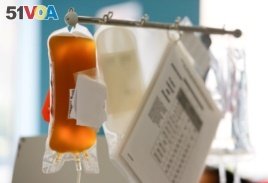
\includegraphics[scale=0.7]{001_voa_20200825.jpg}
\caption{ILE - Convalescent plasma from a recovered coronavirus disease patient.}
\end{figure}
In its announcement, the FDA said, "it is reasonable to believe that COVID-19 convalescent plasma may be effective in lessening the severity or shortening the length of COVID-19 illness in some hospitalized patients." The agency said that more human trials are needed, "as COVID-19 convalescent plasma does not yet represent a new standard of care based on the current available evidence."
Soumya Swaminathan is Chief Scientist at the WHO. She said only a few human trials of convalescent plasma have produced results. "At the moment, it's still very low-quality evidence," Swaminathan told reporters Monday.
The WHO said one Chinese study showed plasma from people who have recovered from coronavirus failed to make a difference in hospitalized patients, while another showed it can lower the risk of death.
What is convalescent plasma?
The treatment involves giving plasma from recovered COVID-19 patients to sick ones. Plasma is the liquid part of blood. Plasma from recovered patients is filled with antibodies, proteins that can kill harmful viruses and bacteria.
The treatment was used during the 1918 flu pandemic. It was also used to fight several other infections before modern medicine found new anti-viral drugs.
Earlier this month, researchers at the Mayo Clinic, in Minnesota, reported data from its experimental program to treat COVID-19 patients around the U.S. with convalescent plasma.
The program called "Expanded Access Program" was not an official study. It did not provide enough information to guarantee that the treatment cured COVID-19. It was "designed to increase access to investigational convalescent plasma and evaluate the safety of this experimental therapy."
The health organization said 70,00 patients received the treatment. It found fewer deaths among those who received the plasma within three days of COVID-19 diagnosis.
Dr. Michael Joyner is lead researcher for the program. He said, "Our hope is that the safety findings and possible efficacy signals could inform the body of knowledge about the use of convalescent plasma to modify the course of COVID-19."
I'm Caty Weaver.
Hai Do wrote this story for Learning English with additional reporting from Reuters and the Associated Press. Caty Weaver was the editor.

\begin{messagebox}
Words in This Story
convalescent - adj. recovering from an illness
plasma - n. the watery part of blood that contains blood cells
illness - n. a condition of being unhealthy, sick
standard - n. a level quality or achievement that is considered acceptable
pandemic - n. an occurrence in which a disease spreads very quickly and affects a large number of people around the world
access - n. a way of getting something
evaluate - v. to judge the value or condition carefully
\end{messagebox}

\paragraph{\href{https://www.51voa.com/VOA\_Special\_English/covid--plasma-a-breakthrough-or-an-experiment-85234_1.html}{翻译}}

Convalescent plasma, which has long been used to treat diseases, has become the latest issue in the race to find treatment for COVID-19.
长期以来一直被用于治疗疾病的康复者血清已经成为了寻找新冠肺炎疗法竞赛中的最新话题。
On Sunday, President Donald Trump announced that the United States would permit the emergency use of convalescent plasma to treat COVID-19 patients. Trump called it "a breakthrough."
川普总统周日宣布,美国将批准康复者血清用于治疗新冠肺炎患者的紧急使用。川普称其为“一次突破。”

However, the World Health Organization (WHO) on Monday warned that the treatment is still experimental. The group described the evidence in support of the treatment as "low quality."
然而,世卫组织周一警告说,这种疗法仍然处于试验阶段。该组织称这种疗法的支持证据“质量不高。”

Trump made the plasma announcement after his administration accused the U.S. Food and Drug Administration (FDA) of delaying in order to hurt his re-election chances this November.
在川普政府指责美国食品药品监督管理局故意拖延以损害他今年11月的连任机会之后,川普发布了这篇血清通告。

The emergency approval makes it easier for some patients to get the treatment. However, it is not the same as full FDA approval for treatment.
这次紧急批准使得一些患者更容易接受到这种治疗。然而,这与美国食品药品监督管理局完全批准这种疗法有所区别。

In its announcement, the FDA said, "it is reasonable to believe that COVID-19 convalescent plasma may be effective in lessening the severity or shortening the length of COVID-19 illness in some hospitalized patients." The agency said that more human trials are needed, "as COVID-19 convalescent plasma does not yet represent a new standard of care based on the current available evidence."
美国食品药品监督管理局在声明中表示,“有理由相信,新冠肺炎康复者血清可以有效减轻某些住院患者的病情或缩短其病程。”该机构表示,还需要进行更多人体试验,“因为根据现有证据,新冠肺炎康复者血清尚不能代表一种新的治疗标准。”

Soumya Swaminathan is Chief Scientist at the WHO. She said only a few human trials of convalescent plasma have produced results. "At the moment, it's still very low-quality evidence," Swaminathan told reporters Monday.
苏米亚·斯瓦米纳坦是世卫组织的首席科学家。她表示,只有少数几项关于康复者血清的人体试验产生了效果。斯瓦米纳坦周一对记者表示:“目前,这仍然算非常低质量的证据。”

The WHO said one Chinese study showed plasma from people who have recovered from coronavirus failed to make a difference in hospitalized patients, while another showed it can lower the risk of death.
世卫组织表示,中国的一项研究表明,来自新冠病毒康复者的血清未能让住院患者产生差异,而另一项研究表明,它可以降低死亡风险。

What is convalescent plasma?
什么是康复者血清?

The treatment involves giving plasma from recovered COVID-19 patients to sick ones. Plasma is the liquid part of blood. Plasma from recovered patients is filled with antibodies, proteins that can kill harmful viruses and bacteria.
这种疗法将新冠肺炎康复者的血清注射给患病患者。血清是血液的液体部分。康复者血清中充满了可以杀死有害病毒和细菌的抗体和蛋白质。

The treatment was used during the 1918 flu pandemic. It was also used to fight several other infections before modern medicine found new anti-viral drugs.
这种疗法在1918年的大流感期间被使用过。在现代医学发现新的抗病毒药物之前,它还被用于抵抗另外几种感染。

Earlier this month, researchers at the Mayo Clinic, in Minnesota, reported data from its experimental program to treat COVID-19 patients around the U.S. with convalescent plasma.
本月初,明尼苏达州梅奥诊所的研究人员报告了一项实验项目中的数据,该项目利用康复者血清治疗美国各地的新冠肺炎患者。

The program called "Expanded Access Program" was not an official study. It did not provide enough information to guarantee that the treatment cured COVID-19. It was "designed to increase access to investigational convalescent plasma and evaluate the safety of this experimental therapy."
这项被称为“Expanded Access Program”的项目并非官方性质的研究。它没有提供足够信息来保证这种疗法可以治愈新冠肺炎。它的目的是“推动康复者血清的调查并评估这种试验疗法的安全性。”

The health organization said 70,00 patients received the treatment. It found fewer deaths among those who received the plasma within three days of COVID-19 diagnosis.
这家卫生机构表示,有7千名患者接受了这种治疗。该机构发现,在新冠肺炎确诊3天内接受这种血清治疗的患者的死亡率更低。

Dr. Michael Joyner is lead researcher for the program. He said, "Our hope is that the safety findings and possible efficacy signals could inform the body of knowledge about the use of convalescent plasma to modify the course of COVID-19."
迈克尔·乔伊纳博士是该项目的首席研究员。他说:“我们希望这种安全结论和可能疗效信号可以提供关于使用康复者血清改变新冠肺炎病程的主体知识。”
\paragraph{\href{https://files.21voa.com/202008/covid-19-plasma-a-breakthrough-or-an-experiment.mp3}{音频}}

